\chapter{Verification and Validation}
\section{Verification by the Method of manufactured solutions}
To ensure the correctness of the newly implemented system with the magnetic vector potential $A_\parallel$, a test model has been set up with the method of manufactured solutions (MMS) \cite{ManufacturedSolution}. This allows to directly compare the numerical and analytic solutions and therefore validate the implementation and verify the order of convergence of the numerical operators. 

\subsection{Test system}
The MMS test model is a fraction of a torus with a circular cross-section with an inner radius of 0.48m, an outer radius of 2.72m and a simulated plasma edge width of 0.64m. An example of the 3D mesh geometry is shown in \autoref{fig:MMSModelScheme}. To test the information exchange between zones in the model topology from \autoref{ssec:SpatialDiscretization}, each coordinate direction is split in two zones totaling to 8 zones.

\begin{figure}[H]
	\centering
	\begin{subfigure}[b]{0.4\textwidth}
		\centering
		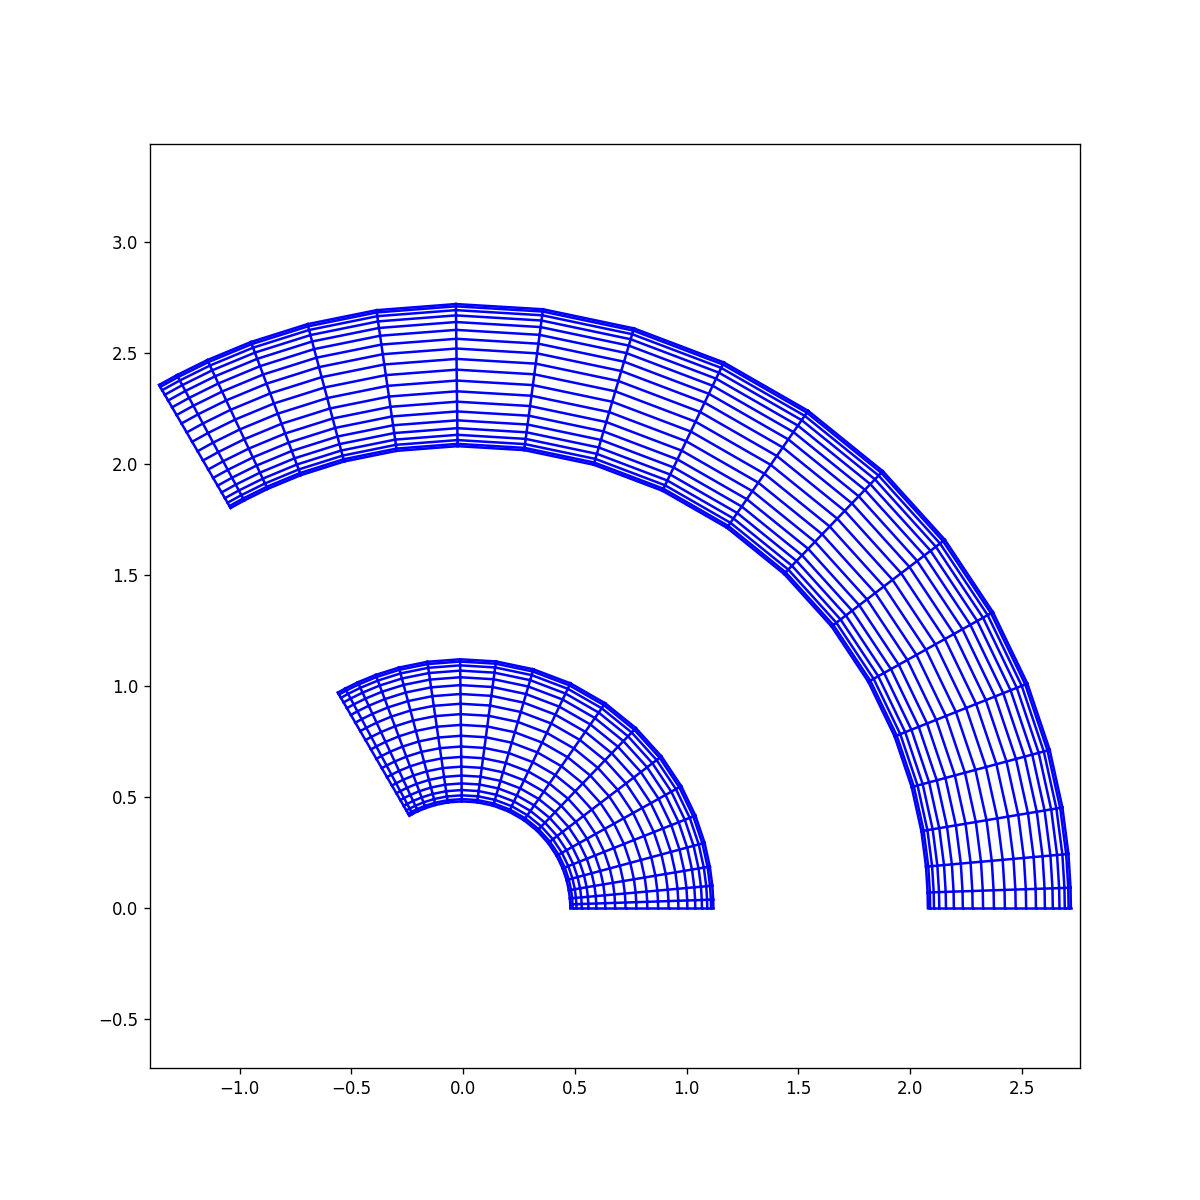
\includegraphics[width=1\textwidth]{schemes/torturedGrid_r_phi_view.png}
		\subcaption{Top view of the $\psi-\varphi$ plane \\ \textit{the two bands correspond to \\ the poloidal angles $0$ and $\pi$}}
		\label{fig:MMSModelTorturedTopView}
	\end{subfigure}
	\begin{subfigure}[b]{0.4\textwidth}
		\centering
		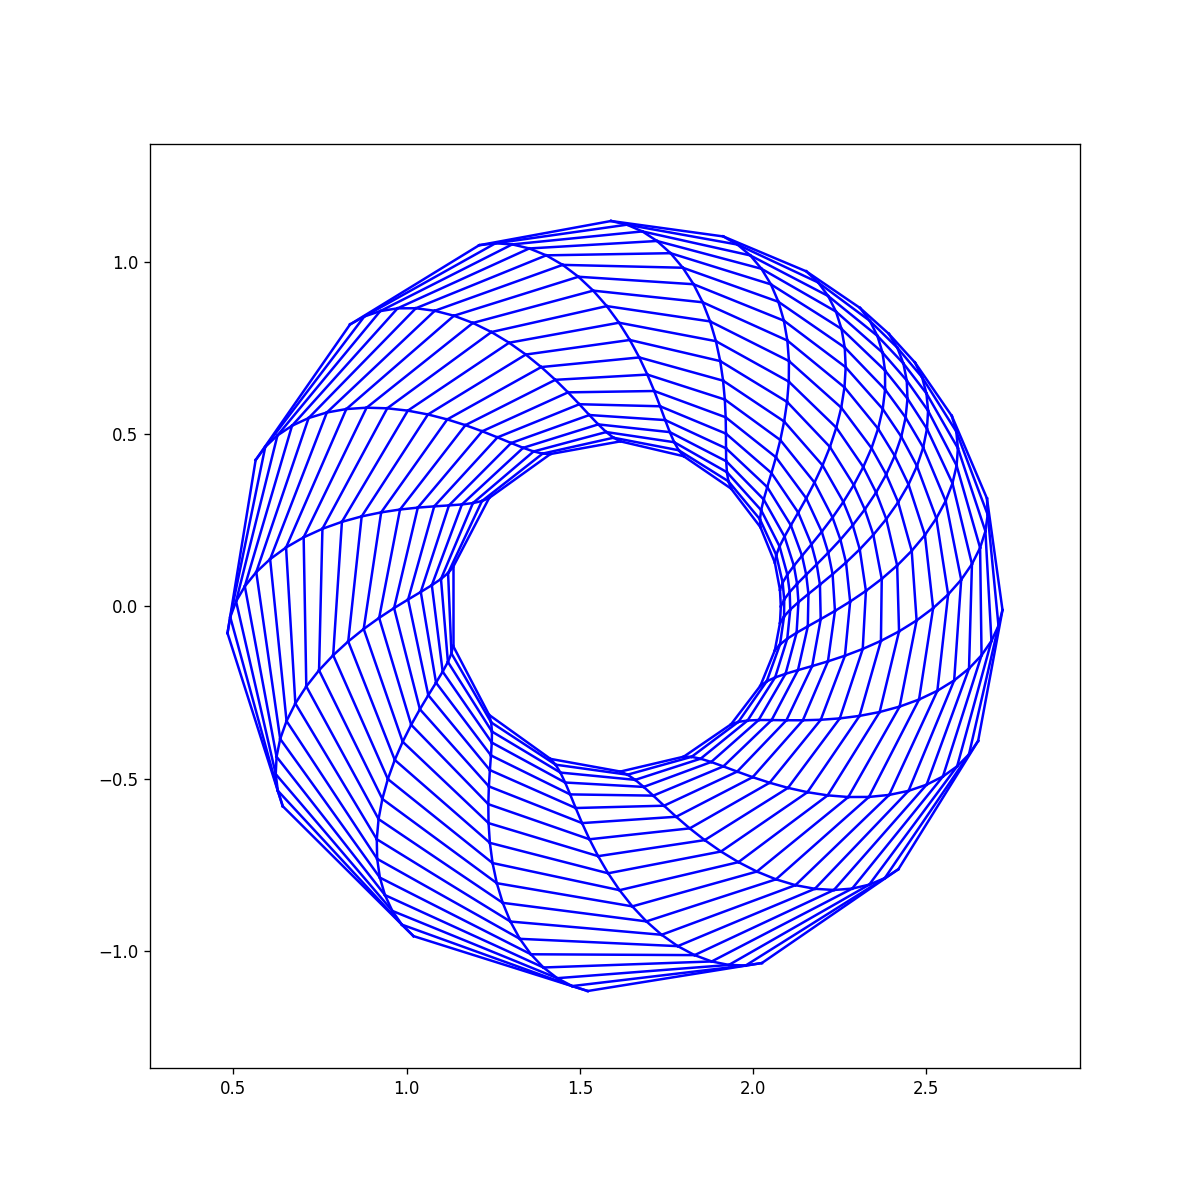
\includegraphics[width=1\textwidth]{schemes/torturedGrid_r_theta_view.png}
		\subcaption{View of a cross-section of the torus in the $\psi-\theta$ plane \\ \textit{The cross-section is at $\varphi=0$}}
		\label{fig:MMSModelTorturedCrossSection}
	\end{subfigure}	
	\caption{Distorted MMS mesh geometry with $N=20$ cells per dimension on a 3rd of a torus}
	\label{fig:MMSModelScheme}
\end{figure}

In the MMS geometry, $\psi$ denotes the radius of the tube and $R$ the radius of the entire torus. If $aR_0=1.6$ is the distance of the tube center to the torus center, we have:
$$  R = aR_0 + \psi\cdot\cos(\theta) $$
Together with the poloidal coordinate $\theta\in[0,2\pi]$ and the toroidal coordinate $\varphi\in[0,2\pi/N_{div}]$ where $1/N_{div}$ is the considered fraction of the torus, each point in the domain is uniquely described by the curvilinear coordinates $[\psi,\theta,\varphi]$. 
We can define some $\vec{P} = [X,Y,Z]^T$ in a cartesian basis of the 3D domain:

\begin{align*}
	X &= R\cos(\varphi) &  Y &= \psi\cdot\sin(\theta)  &  Z &= R\sin(\varphi)
\end{align*} 
In this setting, the basis vectors of the curvilinear coordinates from \autoref{ssec:MetricCurvilinearCoordinates} can be calculated analytically. The covariant basis vectors are:
\begin{align*}
	\vec{e}_\psi &= \pdv{\vec{P}}{\psi} = \begin{bmatrix} \cos(\theta)\cos(\varphi) \\ \sin(\theta) \\ \cos(\theta)\sin(\varphi) \end{bmatrix} & \vec{e}_\theta &= \pdv{\vec{P}}{\theta} = \begin{bmatrix} -\psi\sin(\theta)\cos(\varphi) \\ \psi\cos(\theta) \\ -\psi\sin(\theta)\sin(\varphi) \end{bmatrix} & \vec{e}_\varphi &= \pdv{\vec{P}}{\varphi} = \begin{bmatrix} -Z \\ 0 \\ X \end{bmatrix}
\end{align*}
We can further calculate the metric coefficients:
$$ g_{ij} = \vec{e}_i\cdot\vec{e}_j
= \begin{bmatrix}
	1 & 0 & 0 \\ 0 & \psi^2 & 0 \\ 0 & 0 & R^2
\end{bmatrix} \qquad \text{and} \qquad J = \sqrt{\det[g_{ij}]} = \psi R$$
 
As generally required by S3X, the magnetic field is axisymmetric and thus does not depend on the toroidal coordinate $\varphi$. By construction, it only has a poloidal and a toroidal component but no radial component, which are given in \autoref{eq:MMSMagneticField}.

\begin{equation}
	\label{eq:MMSMagneticField}
	\begin{cases}
		B_\theta = \frac{1}{aR}\Psi_0 & \text{poloidal magnetic field}  \\
		B_\varphi = \frac{R_0}{R}B_0 & \text{toroidal magnetic field}
	\end{cases}
\end{equation}

The magnetic field parameters are chosen such that the ratio of toroidal over poloidal magnetic field strength is $aR_0B_0/\Psi_0 = 12$. 
Tests have been performed on various mesh geometries in the scope of S3X from a perfectly regular grid with equally spaced cells in all coordinate directions to the distorted mesh depicted above. As the program can be either executed in a 2D or 3D mode with adapted stencils and geometry calculations, MMS tests have been developed for both scenarios.

\subsection{Analytic solution}

We are interested in the vorticity system on the electric potential $\Phi$ and the parallel magnetic vector potential $A_\parallel$. We postulate that their analytic form is: 
\begin{align}
	\Phi =& \Phi_0 \left(1 + 0.1 \cos(\theta)\cos(\frac{\varphi}{N_{div}})\sin(2\pi \frac{\psi-\psi_{min}}{\psi_{max} - \psi_{min}}) \right) \\
	A_\parallel =& A_{\parallel,0} \left(1 + 0.1 \cos(\theta)\cos(\frac{\varphi}{N_{div}})\sin(2\pi \frac{\psi-\psi_{min}}{\psi_{max} - \psi_{min}}) \right)
	\label{eq:MMSAnalyticFormPhiAPara}
\end{align}

A similar expression is chosen for the densities $n_{i/e}$ and temperatures $T_{i/e}$ that also contribute to the vorticity equation. The entire form of the test equation is:

\begin{align}
	&\begin{cases}
		\partial_t\vec{\grad}\cdot\left(\frac{m_in_i}{B^2}\vec{\grad}_\perp\Phi\right) + \vec{\grad}\cdot\sigma_\parallel \left(\grad_\parallel\Phi\vec{b}+\partial_t A_\parallel\right) &= \partial_t \Omega_\pi + \vec{\grad}\cdot\sigma_\parallel\left( + \frac{T_e}{e}\grad_\parallel \log(n_e)\vec{b} + \frac{1.71}{e}\grad_\parallel T_e\vec{b}\right)  - S^{MMS}_\Phi \\
		\qquad \vec{\grad}\cdot\left(\vec{\grad}_\perp A_\parallel\vec{b}\right) - \mu_0 \sigma_\parallel \left( \grad_\parallel \Phi + \partial_t A_\parallel\right)&= -\mu_0 \sigma_\parallel \left(\frac{T_e}{e}\grad_\parallel \log(n_e) + \frac{1.71}{e}\grad_\parallel T_e\right) - S^{MMS}_{A_\parallel}
	\end{cases} \nonumber \\
	&\Omega_\pi = \vec{\grad}\cdot\left(\frac{m_i}{Z_iB^2}\vec{\grad}_\perp[nT]\right)
	\label{eq:MMSTestSystem}
\end{align}

The main difference to the original system of equations in \autoref{eq:vorticityEquation_electromagnetic} are the MMS source terms $S^{MMS}_\Phi$ and $S^{MMS}_{A_\parallel}$. They contain the analytic evaluation of all other time-independant terms in the respective line of the equation. The derivatives on curvilinear coordinates can be calculated analytically with the metric theory discussed in \autoref{ssec:MetricCurvilinearCoordinates}. Boundary conditions are enforced by a penalty method on the boundary cell layer where the two quantities are set to their analytic expression. The MMS system is initialized with the analytic expressions for $\Phi$ and $A_\parallel$ in \autoref{eq:MMSAnalyticFormPhiAPara} and uniquely the vorticity equation is solved for one timestep. We are in a steady state, so the numerical solution after the first timestep should be equal to the initial state. \\
One drawback of a steady state system is that time derivatives are always assumed to vanish and terms such as $\Omega_\pi$, the perpendicular Laplacian of $\Phi$ or the divergence of $A_\parallel$ are not confronted to their analytic form. To catch these terms, we add the vorticity $\Omega$ to the MMS system and include it in the subsequent analysis. It is initialized with its analytic form:
$$ \Omega = \Omega_\pi + \vec{\grad}\cdot\left(\frac{m_in_i}{B^2}\vec{\grad}_\perp\Phi\right) + \vec{\grad}\cdot\sigma_\parallel A_\parallel $$
and then calculated numerically after the first timestep. This allows to compare a numerical and an analytic form of the vorticity and hence all terms in \autoref{eq:MMSTestSystem}.

\subsection{Order of convergence}
- \\
- \\
- \\
Describe \\
- \\
- \\
- \\
\begin{figure}[H]
	\centering
	\begin{subfigure}[b]{0.49\textwidth}
		\centering
		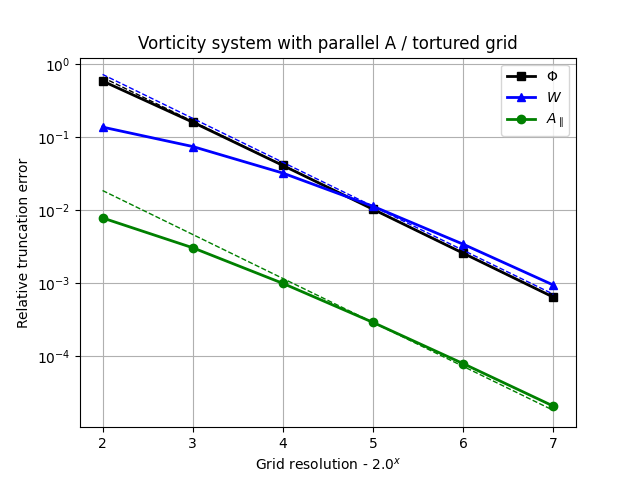
\includegraphics[width=1\textwidth]{schemes/err_rel_vortAParaSystem_grid2_2D.png}
		\subcaption{2D system}
		\label{fig:MMSTorturedVortAPara2DConvergence}
	\end{subfigure}
	\begin{subfigure}[b]{0.49\textwidth}
		\centering
		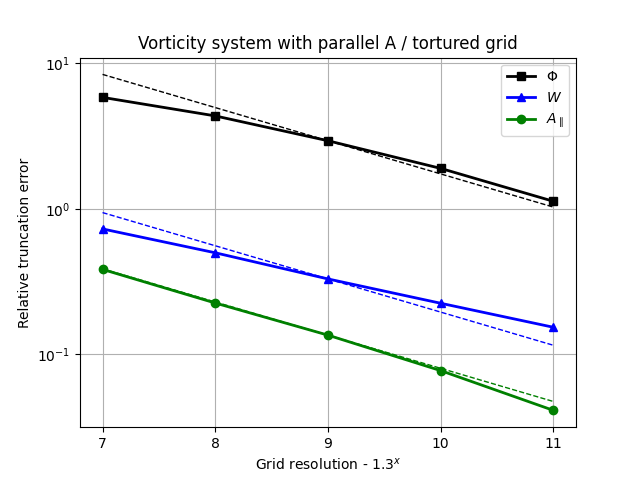
\includegraphics[width=1\textwidth]{schemes/err_rel_vortAParaSystem_grid2_3D.png}
		\subcaption{3D system}
		\label{fig:MMSTorturedVortAPara3DConvergence}
	\end{subfigure}
	\caption{Relative error between the initial plasma and the solution after one timestep. The $x$-axis indicates the number of points per zone in each direction, the total number of points is thus $N_{tot}^{3D} = 8\cdot X^3$ (resp. $N_{tot}^{2D} = 4\cdot X^2$). The dashed lines indicate the slope of the ideal 2nd order convergence}
	\label{fig:MMSTorturedVortAParaConvergence}
\end{figure}
- \\
- \\
this beautiful graph \\ - \\ - \\ Thanks.


\section{Linear Analysis}

.... 
\subsection{Pure advection}
A first step to verify the correct physical behaviour of the simulation would be to investigate the plasma advection equations. \\
For this objective we set up a simplistic plasma model on a rectangular 2D SLAB topology. Periodic boundary conditions in all directions allow to properly observe wave propagation without any inference at the domain boundaries. In an isothermal hydrogen plasma without source terms and drifts, the governing equations then simplify to:

\begin{align}
	\partial_t n_i + \vec{\grad}\cdot\left(n_i\vec{u}_i\right) &= 0 \label{eq:AdvectionLinearAnalysis_ionMass} \\
	n_e &= n_i \label{eq:AdvectionLinearAnalysis_quasiNeutrality} \\
	\partial_t \left(m_in_iu_\parallel\right) + \vec{\grad}\cdot\left(m_in_iu_\parallel u_i\right) &= -2T_e\vec{\grad}_\parallel n_e \label{eq:AdvectionLinearAnalysis_parallelMomentumBalance}
\end{align}

In this simple plasma, only the density and the velocity evolve over time and depend on each other. The electric potential $\Phi$ can also be computed and observed, but it does not interfere with the system because the parallel electric field in the momentum balance \autoref{eq:AdvectionLinearAnalysis_parallelMomentumBalance} is calculated from the electron pressure gradient $E_\parallel = (\vec{\grad}_\parallel p_e + R_e) / n_e$. \\

To perform the linear analysis of the system, we assume that field variables such as the velocity or density respect some Fourier solution as sum of several wave modes with respective amplitudes $\tilde{X}_{\omega,k_\perp,k_\parallel}$:
\begin{equation}
	 X = \bar{X} + \hat{X} = X_0 + \sum\tilde{X}_{\omega,k_\perp,k_\parallel}e^{i(-\omega t + k_\perp \psi + k_\parallel \theta)} \label{eq:FourierModeSolution}
\end{equation}

Electron and ion density are identical because of the quasi-neutrality assumption in \autoref{eq:AdvectionLinearAnalysis_quasiNeutrality}. Since we do not consider any drifts the radial component $u_\psi$ of the velocity vector vanishes. Further, the mean density is $\bar{n}=n_0$ while the mean velocity $\bar{u}_\theta$ is zero. Because we are only interested in a first order approximation of the solution, we neglect all higher-order mixed fluctuating terms. Thus, \autoref{eq:AdvectionLinearAnalysis_ionMass} and \autoref{eq:AdvectionLinearAnalysis_parallelMomentumBalance} transform to:

\begin{align*}
	&&-i\omega\hat{n} + i\bar{n}k_\parallel\hat{u}_\theta + i\bar{u}_\theta k_\parallel\hat{n} &= 0 &\Leftrightarrow&& \hat{u}_\theta &= \frac{\omega}{n_0k_\parallel}\hat{n} \\
	&& -i\omega m_i \left(\bar{n}\hat{u}_\theta + \bar{u}_\theta\hat{n}\right) + im_ik_\parallel\left(2\bar{n}\bar{u}_\theta\hat{u}_\theta + \bar{u}_\theta^2\hat{n}\right) &= -2iT k_\parallel\hat{n}	&\Leftrightarrow&&  \hat{u}_\theta &= \frac{2T k_\parallel}{m_in_0\omega}\hat{n}
\end{align*}

Both are combined to obtain a dispersion relation for the frequency $\omega$:
\begin{align}
	&& \frac{\omega}{n_0k_\parallel} &= \frac{2T k_\parallel}{m_in_0\omega} 
	&\Leftrightarrow&& \omega &= \pm\sqrt{\frac{2T}{m}}k_\parallel \label{eq:AdvectionLinearAnalysis_dispersionRelation}
\end{align}

It is apparent that both solutions for $\omega$ are real therefore non-decaying waves traveling with the speed of sound $c_s = \sqrt{2T/m}$ appear. The perpendicular wave mode does not contribute to the equation so a 1D system along the poloidal axis is sufficient to simulate the behaviour. Both the electron and the ion density are initialized with one sinusoidal perturbation and \autoref{fig:AdvectionSLAB_densityEvolution} shows their evolution. The electron velocity in \autoref{fig:AdvectionSLAB_velocityEvolution} responds to this initial excitation with a shifted standing wave with same frequency. 

\begin{figure}[H]
	\centering
	\begin{subfigure}[b]{0.32\textwidth}
		\centering
		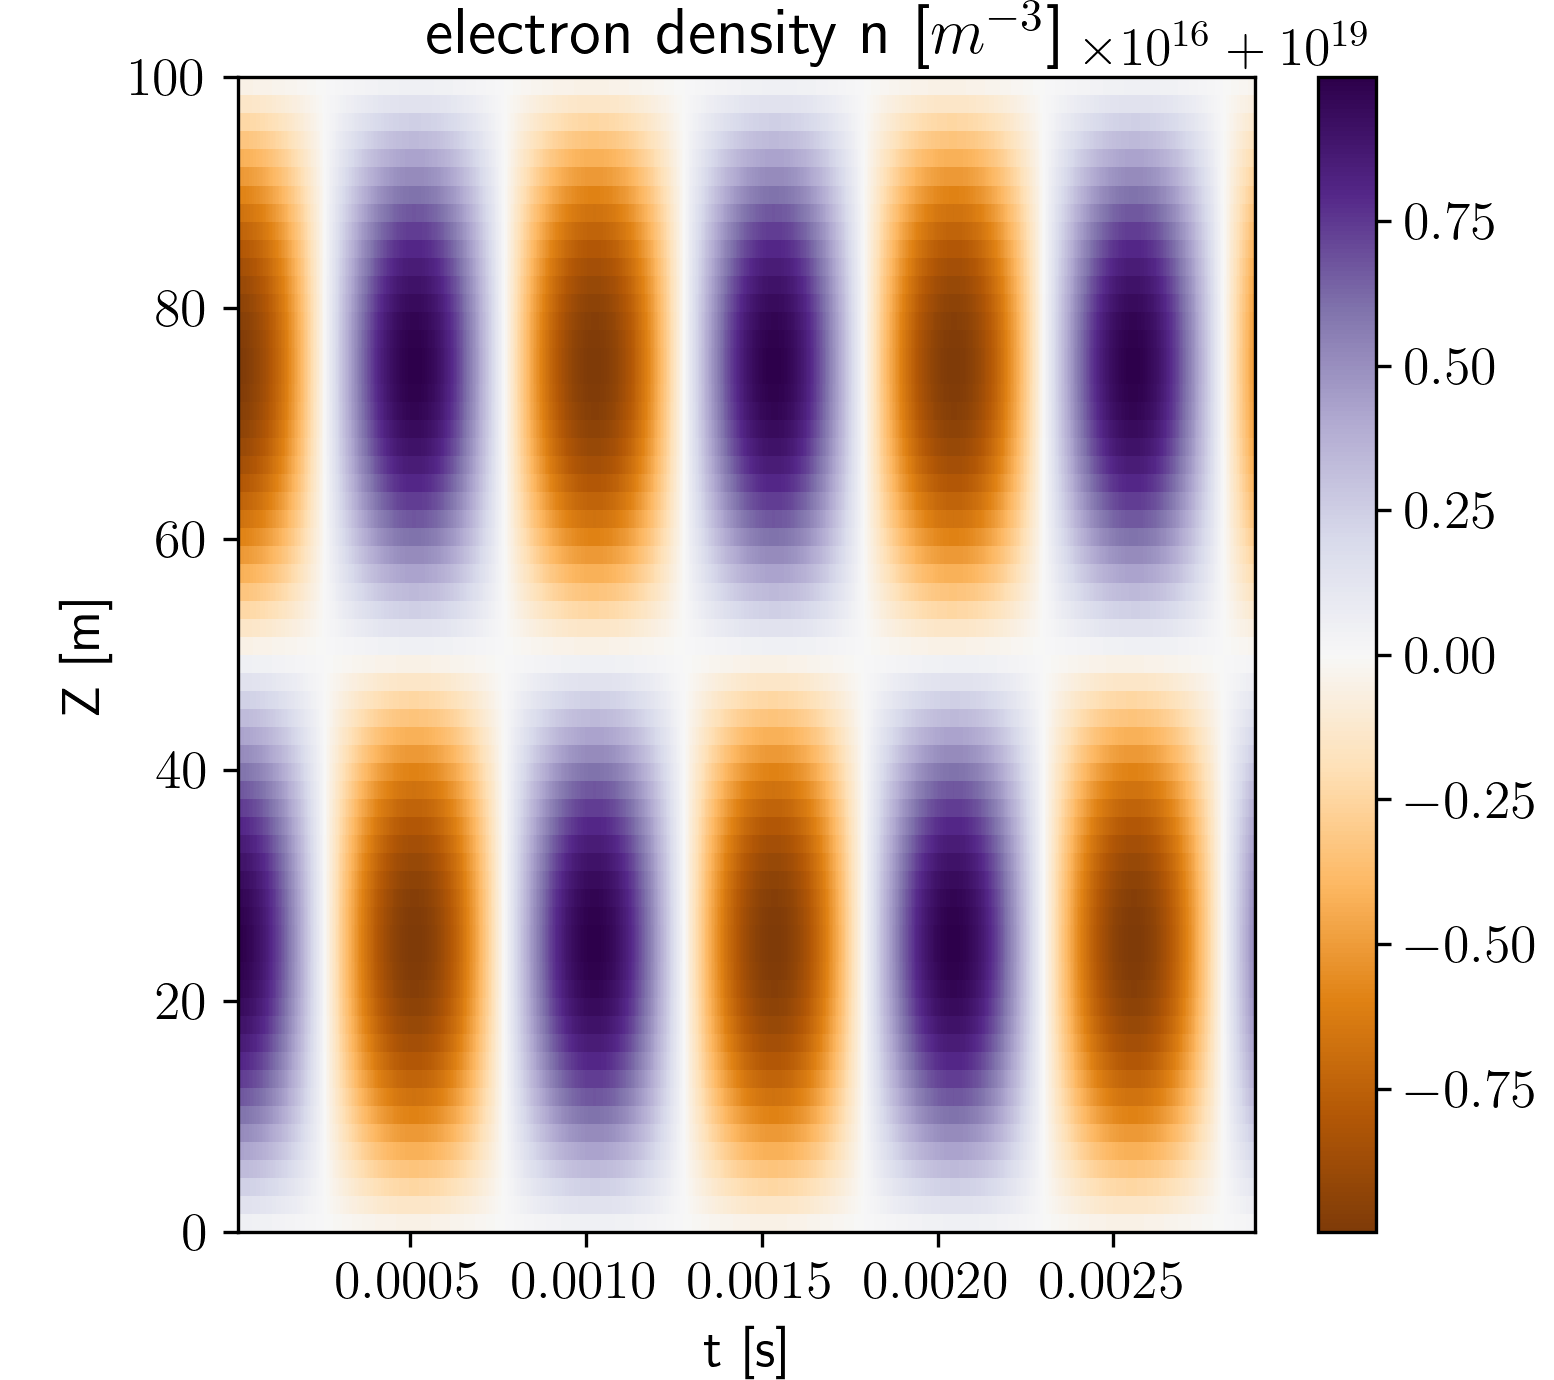
\includegraphics[width=1\textwidth]{schemes/AdvectionSLAB_1D_timeplot_ne.png}
		\subcaption{Evolution of the density \\ \ }
		\label{fig:AdvectionSLAB_densityEvolution}
	\end{subfigure}
	\begin{subfigure}[b]{0.32\textwidth}
		\centering
		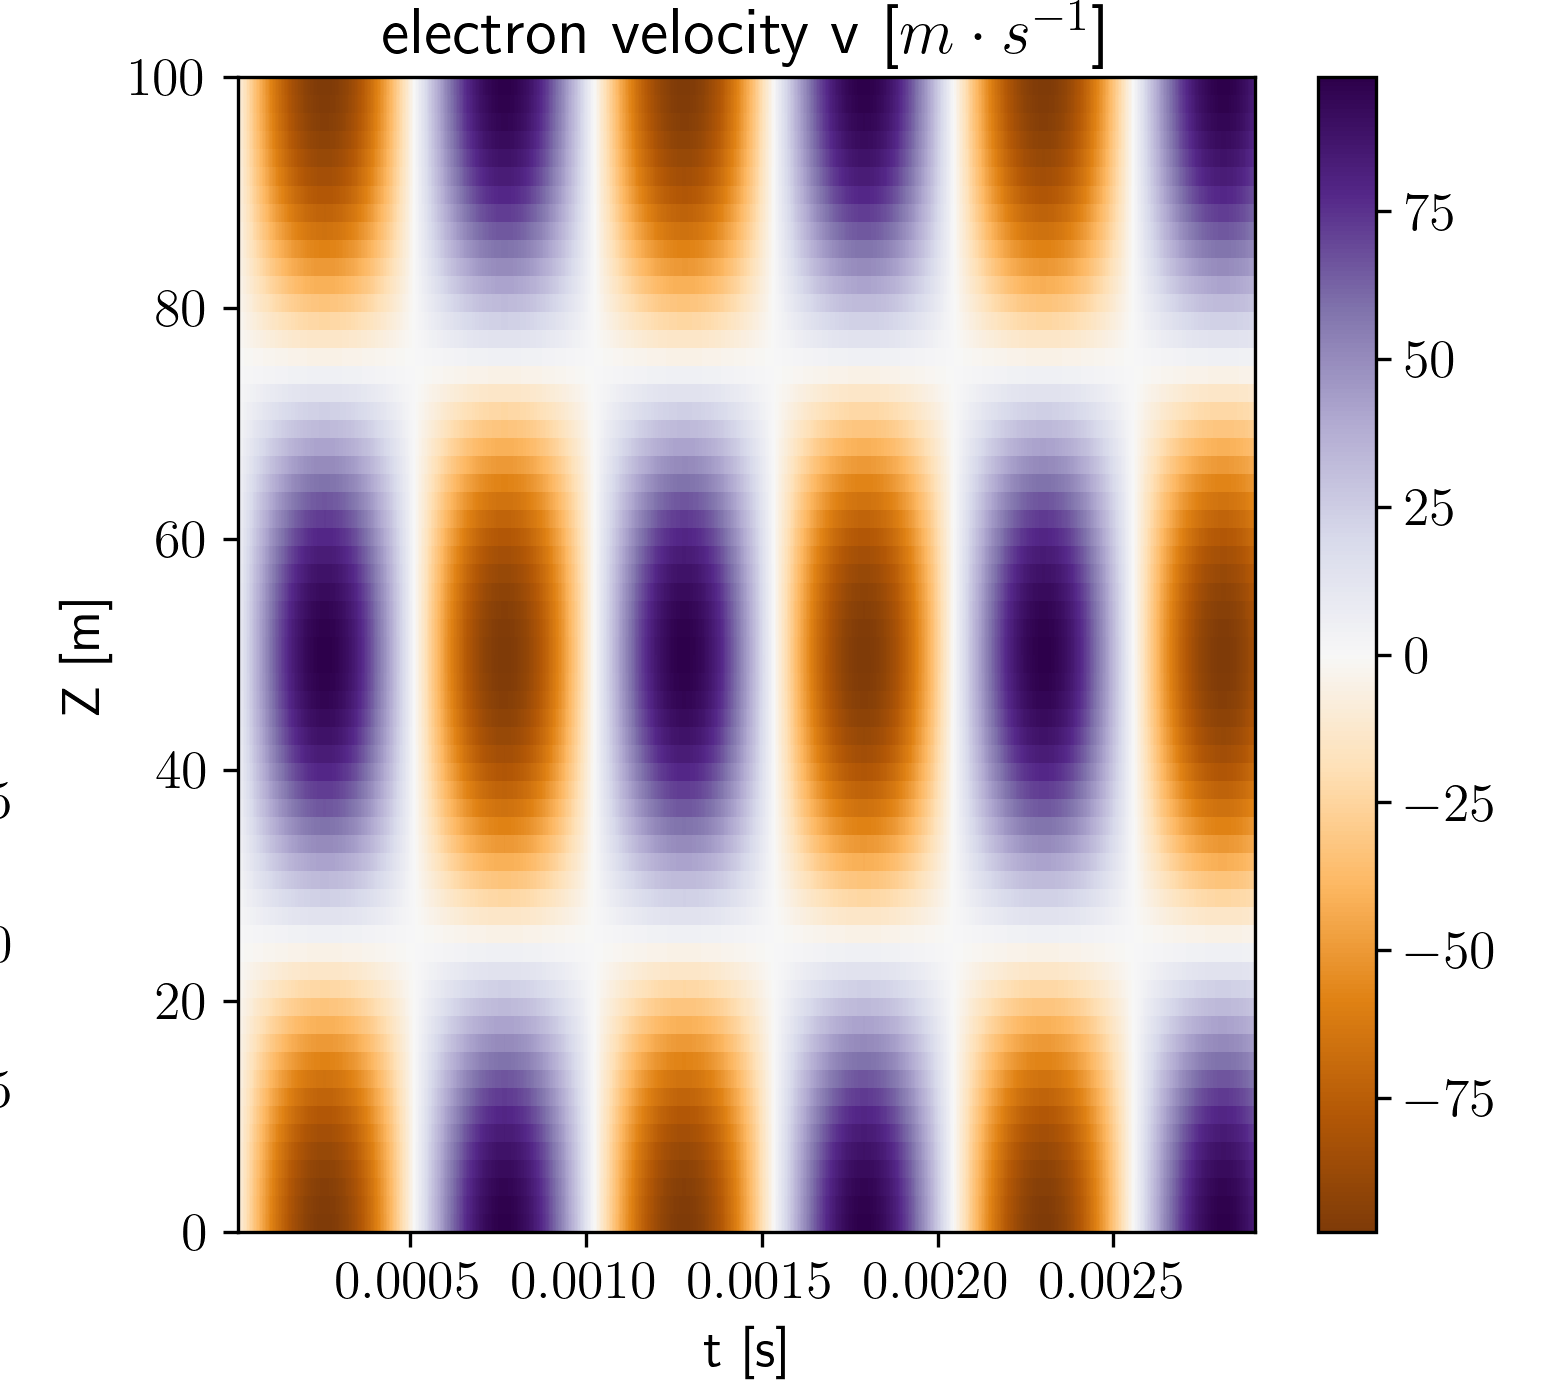
\includegraphics[width=1\textwidth]{schemes/AdvectionSLAB_1D_timeplot_ve.png}
		\subcaption{Evolution of the velocity \\ \ }
		\label{fig:AdvectionSLAB_velocityEvolution}
	\end{subfigure}
	\begin{subfigure}[b]{0.32\textwidth}
		\centering
		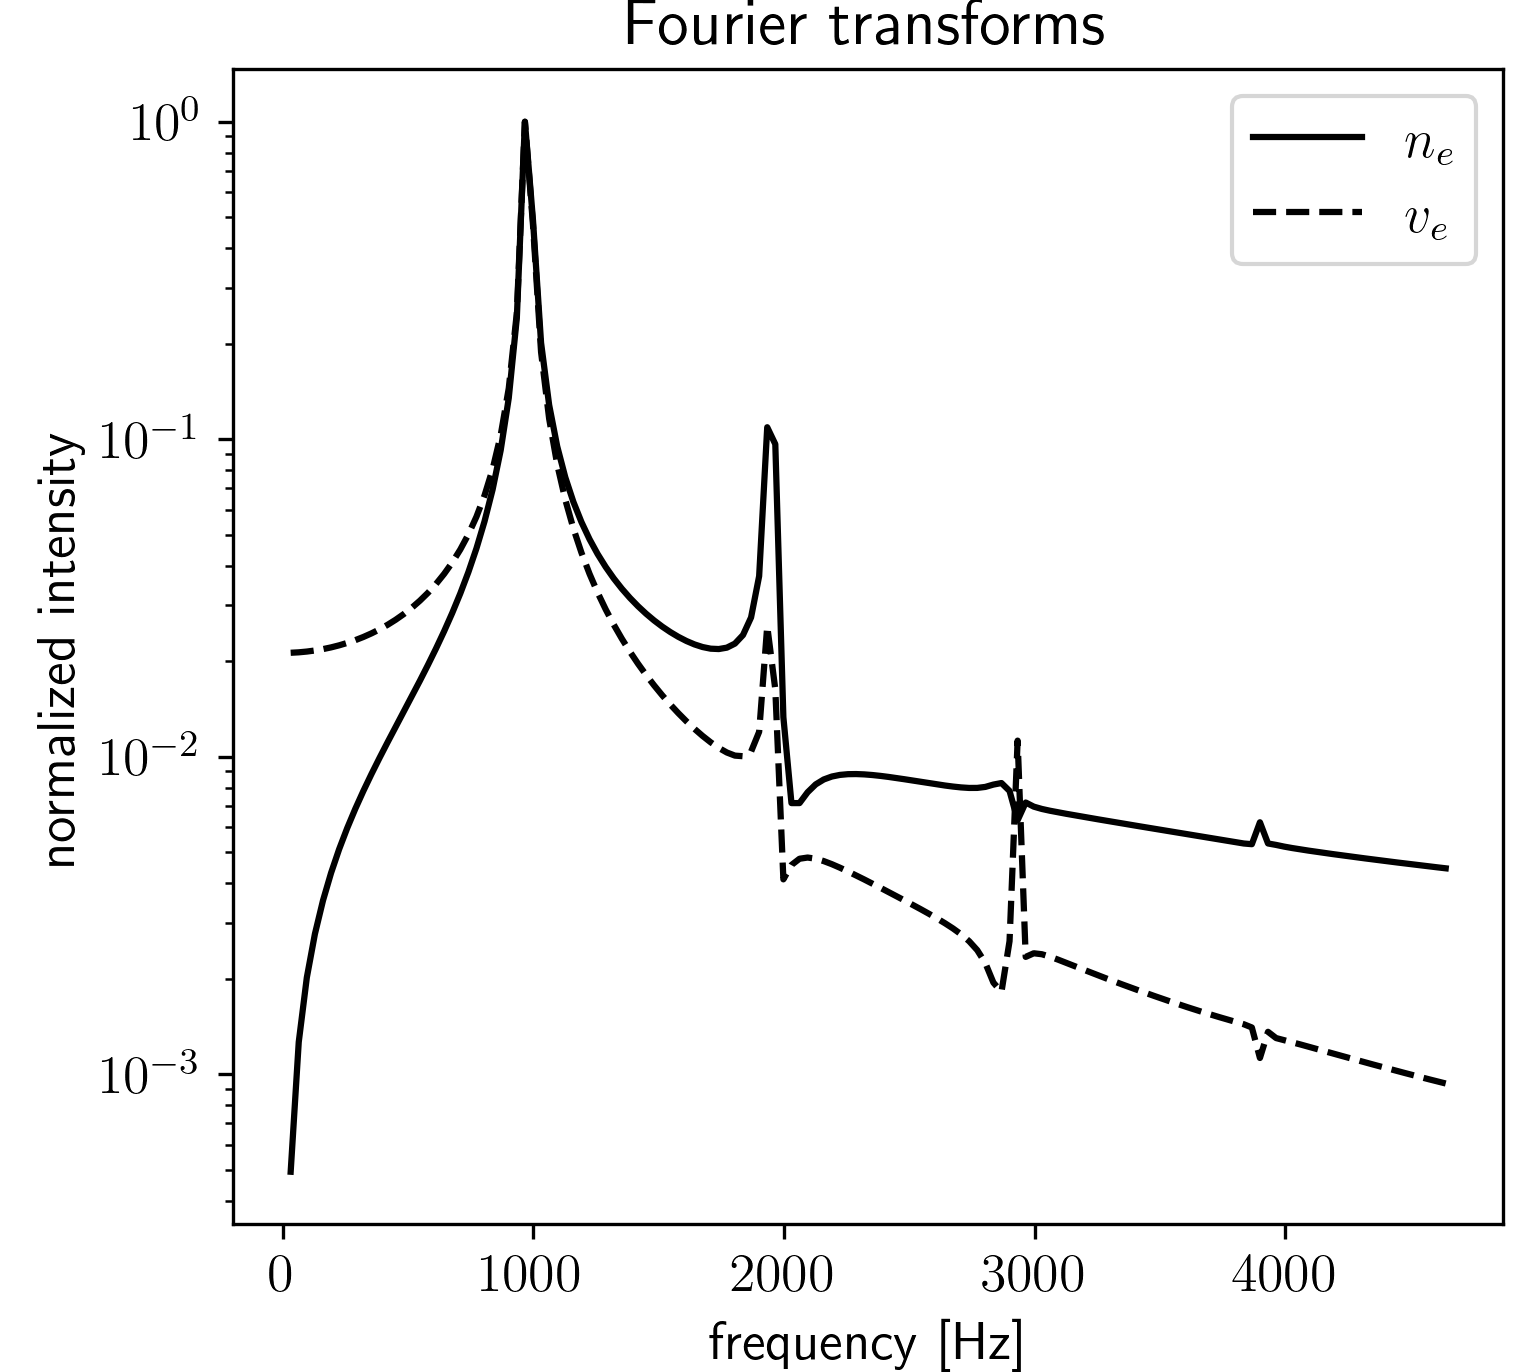
\includegraphics[width=1\textwidth]{schemes/AdvectionSLAB_FFT.png}
		\subcaption{time Fourier transform of the density and velocity}
		\label{fig:AdvectionSLAB_FFT}
	\end{subfigure}
	\caption{Evolution of the 1D SLAB system with 64 cells in poloidal direction over 10000 timesteps with the RK4 scheme. For a better readability only parts of the graphs are represented}
	\label{fig:AdvectionSLAB}
\end{figure}

The system is initialized with one wavemode along the "poloidal" length of $L=100$m so the wavenumber here is $k_\parallel = 2\pi / L \approx 0.0628$. The plasma temperature is kept constant at $T = 100$eV and the mass of a deuterium atom equals to $m_i \approx 3.34\cdot 10^{-27}$kg, so we can expect a system frequency of $\omega\approx 978$Hz from the dispersion relation in \autoref{eq:AdvectionLinearAnalysis_dispersionRelation}. This corresponds precisely to the main frequency peak in \autoref{fig:AdvectionSLAB_FFT} and thus acoustic waves appear in the system as expected. The smaller peaks at higher frequency modes are however not physical and are likely due to numerical noise as their appearance highly depends on the spatial and temporal resolution and their intensity increases for longer simulations. 


\subsection{Electrostatic case}
Before plunging into the vorticity equation with $A_\parallel$ it may be interesting to discuss whether the correct behaviour is actually observed in the original electrostatic implementation. For that we reduce the system to the bare minimum set of equations that involve the electric potential $\Phi$. Neglecting all kind of transport equations and source phenomena remains the following simple equation on $\Phi$: \\
\begin{equation}
		\partial_t\grad\cdot\left[\frac{m_in_i}{B^2}\grad_\perp\Phi\right] = -\grad\cdot\sigma_\parallel\grad_\parallel\Phi \label{eq:AdvectionSLAB_PHI}
\end{equation}

whose simple dispersion relation reads, assuming that $k_\perp \ne 0$:
\begin{align}
	\omega &= -\frac{B^2\sigma_\parallel}{m_in_i}\frac{k_\parallel^2}{k_\perp^2}i &\Rightarrow&& \lambda &= \frac{B^2\sigma_\parallel}{m_in_i}\frac{k_\parallel^2}{k_\perp^2}
\label{eq:AdvectionSLAB_dispersionRelation}
\end{align}

As $\omega$ is a pure negative complex number, we do not expect any oscillations but an exponential decay of the solution. All points in the domain decay with 
\begin{align}
	\Phi(t) = \Phi_0 e^{-\lambda t} + C \label{eq:electrostaticSLABdecay}
\end{align} 
where the decay rate $\lambda$ is the negative imaginary part of $\omega$ and $\Phi_0$ relates to the initial distribution of the electric potential.

The time integration of this system can only be performed by solving the implicit system because there is no direct expression for the time derivative of $\Phi$. Further, the electric potential $\Phi$ appears only in perpendicular and parallel Laplacian operators. Together with the periodic boundary conditions in all directions, one degree of freedom remains and the solution of $\Phi$ can only be calculated up to a constant $C$. To make the system invertible, it is thus necessary to add some term to the system. One simple approach is to fix (or ground) $\Phi$ to a set value $\Phi^G$ at one point $[i_\psi^G, i_\theta^G]$ in the domain. This defines the free parameter $C$ and $\Phi(t)$ at all points converges to $\Phi^G$. 

\begin{figure}[H]
	\centering
	\begin{subfigure}[b]{0.34\textwidth}
		\centering
		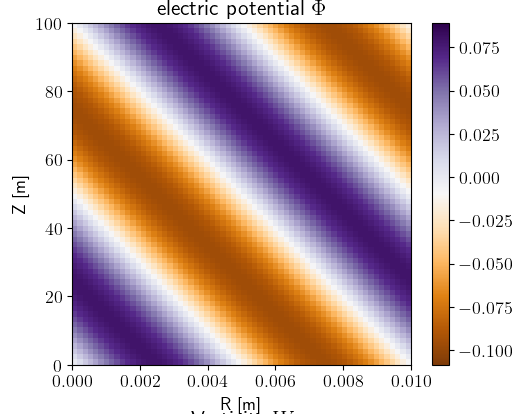
\includegraphics[width=1.\textwidth]{schemes/electrostaticSLAB_1_Phi.png}
		\subcaption{Initial $\Phi(\psi,\theta)$ \\ \ }
		\label{fig:electrostaticSLAB_initialProfile_PHI}
	\end{subfigure}
	\begin{subfigure}[b]{0.34\textwidth}
		\centering
		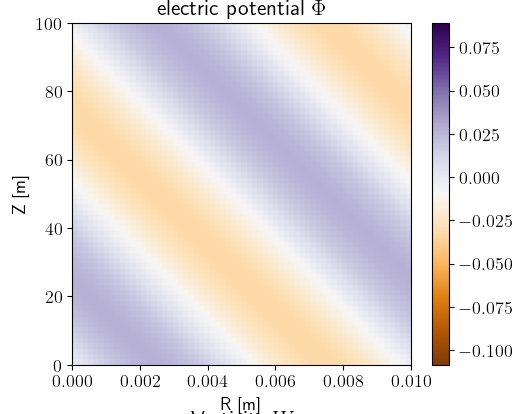
\includegraphics[width=1.\textwidth]{schemes/electrostaticSLAB_35_Phi.png}
		\subcaption{$\Phi(\psi,\theta)$ after 350 timesteps \\ \ }
		\label{fig:electrostaticSLAB_endProfile_PHI}
	\end{subfigure}
	\begin{subfigure}[b]{0.30\textwidth}
		\centering
		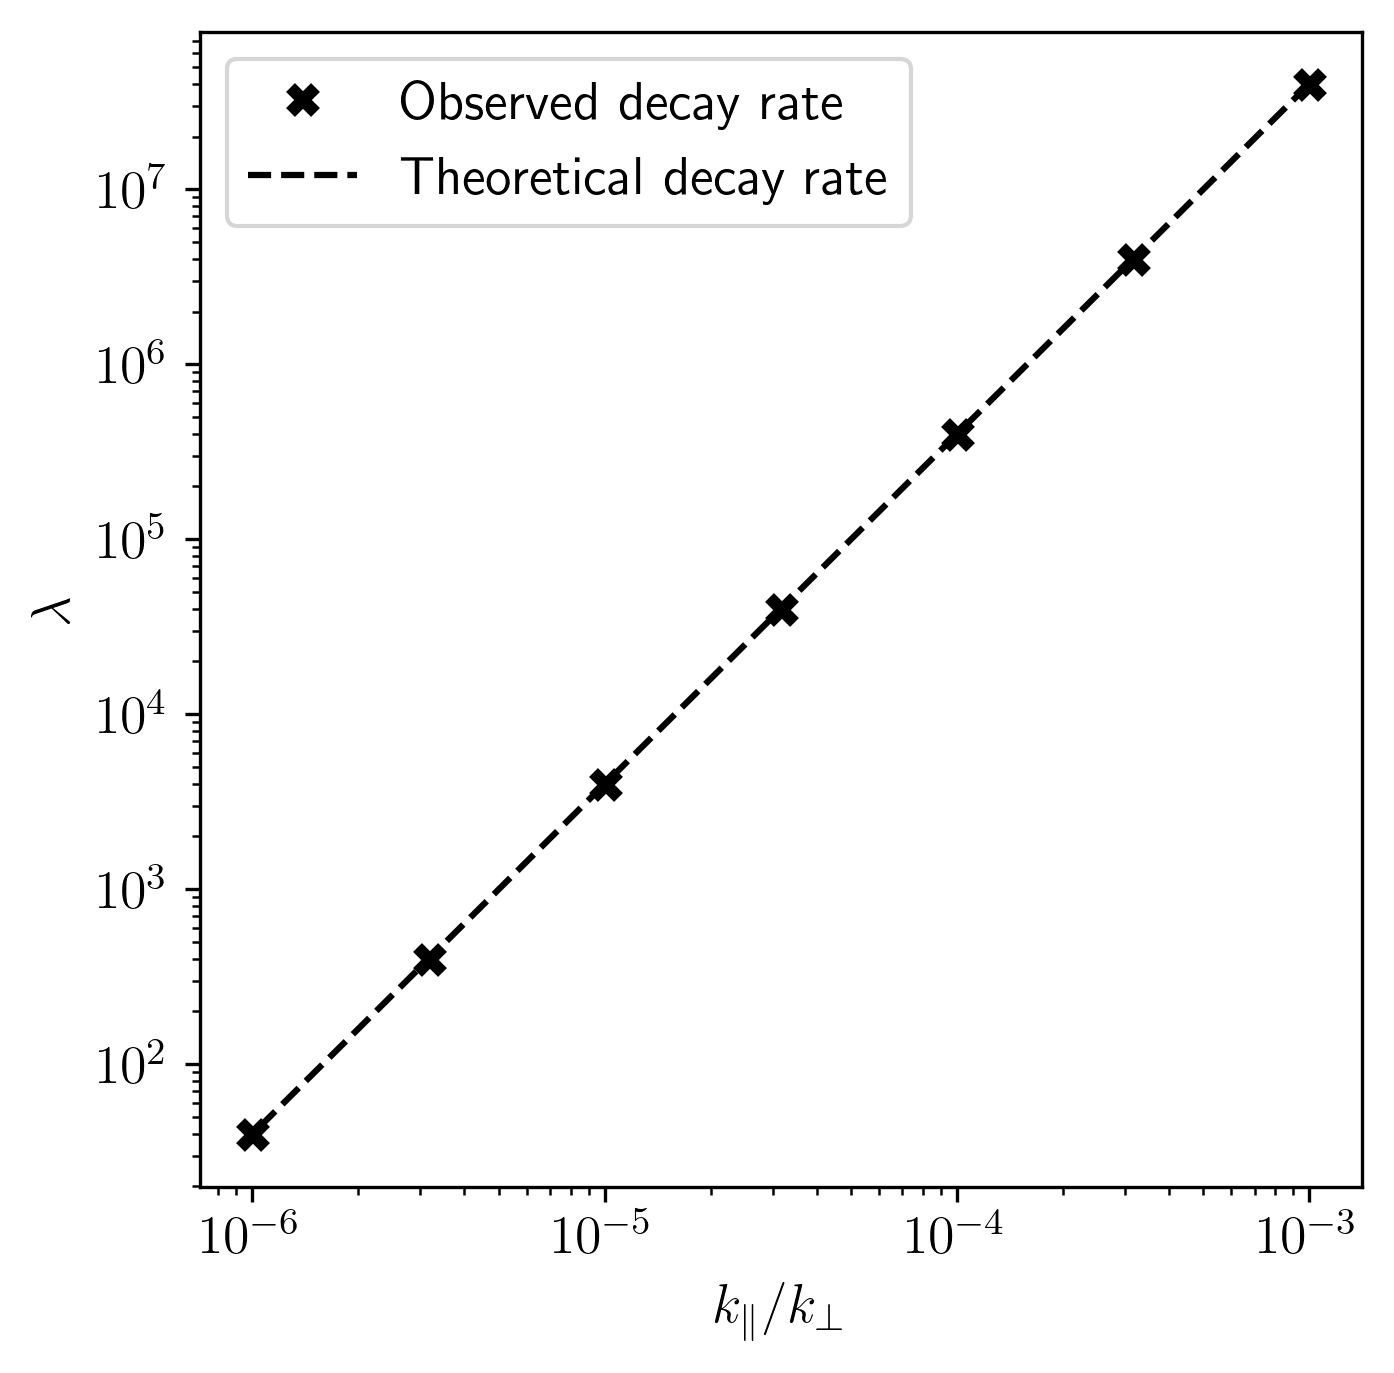
\includegraphics[width=0.95\textwidth]{schemes/Electrostatic_analysis_different_k_para_k_perp.png}
		\subcaption{Estimated decay rates for different wavemodes}
		\label{fig:electrostaticSLAB_decayRateFit}
	\end{subfigure}
	\caption{Evolution of the 2D electrostatic SLAB system with 64 cells in radial and poloidal direction over 10000 timesteps with the implicit Euler scheme. The system is grounded at the center of the domain to $\Phi^G = 0$V.}
	\label{fig:electrostaticSLAB}
\end{figure}

The uniform decay can be clearly seen between \autoref{fig:electrostaticSLAB_initialProfile_PHI} and \autoref{fig:electrostaticSLAB_endProfile_PHI}. It remains to investigate whether the observed attenuation matches the expected decay rate $\lambda$. A Fourier transformation as to determine oscillatory modes for the standing acoustic waves in the previous section is not of great help here, instead we use a non-linear least squares to fit the time evolution of $\Phi(t)$ at an arbitrary point in the domain except the grounded point. We fit the parameters $\Phi_0$, $\lambda$ and $C$ from \autoref{eq:electrostaticSLABdecay} to the simulation data and compare the hence estimated $\lambda$ to the theoretical decay rate for the given initial wave. \autoref{fig:electrostaticSLAB_decayRateFit} shows that there is a strong agreement between the theoretical and fitted decay rates for a large array of domain configurations. The wavenumbers $k_\parallel$ and $k_\perp$ were modified by changing the poloidal respectively the radial size of the domain with always the first wave mode spanning the entire domain. We can safely claim that the original electrostatic implementation produces the expected physical behaviour.

\subsection{Electromagnetic case}
While acoustic waves are characteristic for a physical medium, Alfvén waves dominate oscillations of ions within a magnetic field. The motion occurs in direction of the magnetic field lines where the ion mass accounts for the inertia and the magnetic field tension for the restoring wave force. The Alfvén wave group velocity for a species $i$ is given by:

\begin{equation}
	v_A = \frac{B}{\sqrt{m_in_i\mu_0}} \label{eq:AlfvenGroupVelocity}
\end{equation}

With the new parallel magnetic vector potential $A_\parallel$ into the vorticity \autoref{eq:vorticityEquation_electromagnetic} Alfvén waves should appear in the simulation and the aim of this section is to prove their existence. We follow the same approach as in the previous section for the electrostatic case and reduce the system to the strict necessary minimum and keep following equations: 
\begin{align}
	\partial_t\grad\cdot\left[\frac{m_in_i}{B^2}\grad_\perp\Phi\right] &= \grad\cdot\sigma_\parallel\left(-\grad_\parallel\Phi-\partial_tA_\parallel\right) \label{eq:electromagneticSLAB_PHI} \\
	\Delta_{\perp}A_\parallel &= -\mu_0\sigma_\parallel\left(-\grad_\parallel\Phi-\partial_tA_\parallel\right) \label{eq:electromagneticSLAB_APara}
\end{align}

We ignore any kind of advection phenomena thus all densities $n_{i/e}$ and temperatures $T_{i/e}$ keep their initial uniform distributions their gradients vanish. If we perform the linear analysis of the remaining system we get following relation for \autoref{eq:electromagneticSLAB_PHI}:
\begin{align*}
	&&i\frac{m_in_i}{B^2}k_\perp^2\omega\hat{\Phi} &= \sigma_\parallel k_\parallel^2\hat{\Phi}-\sigma_\parallel k_\parallel\omega\hat{A}_\parallel \\
	&\Leftrightarrow& \hat{A}_\parallel &= \left(\frac{k_\parallel}{\omega} - i\frac{m_in_ik_\perp^2}{\sigma_\parallel B^2k_\parallel}\right)\hat{\Phi}
\end{align*}

and for \autoref{eq:electromagneticSLAB_APara}:
\begin{align*}
	&&-k_\perp^2\hat{A}_\parallel &= i\mu_0\sigma_\parallel k_\parallel\hat{\Phi} - i\mu_0\sigma_\parallel\omega\hat{A}_\parallel \\
	&\Leftrightarrow&\hat{A}_\parallel &= \frac{\mu_0\sigma_\parallel k_\parallel}{\mu_0\sigma_\parallel\omega + i k_\perp^2}\hat{\Phi}
\end{align*}

If we combine both expressions we can relate the frequency to the parallel and perpendicular wave modes:
\begin{align}
	&& \frac{k_\parallel}{\omega} - i\frac{m_in_ik_\perp^2}{\sigma_\parallel B^2k_\parallel} &= \frac{\mu_0\sigma_\parallel k_\parallel}{\mu_0\sigma_\parallel\omega + i k_\perp^2} \nonumber \\
	&\Leftrightarrow& i\frac{m_in_ik_\perp^2\omega}{\sigma_\parallel B^2k_\parallel^2} &= 1- \frac{\mu_0\sigma_\parallel\omega}{\mu_0\sigma_\parallel\omega + i k_\perp^2} \nonumber \\
	&\Leftrightarrow& \omega^2 + i\frac{k_\perp^2\omega}{\mu_0\sigma_\parallel} &= \frac{B^2}{m_in_i\mu_0}k_\parallel^2 \nonumber
\end{align}
We find the square of the Alfvén group velocity \ref{eq:AlfvenGroupVelocity} as a factor before the parallel wave number. There is an additional imaginary term in the dispersion relation which depends on the perpendicular wave number and adds some damping to the system. Let us call $\gamma = 1/(\mu_0\sigma_\parallel)$ the associated damping coefficient. The dispersion relation can then be rewritten to: 

\begin{equation}
	\omega^2+i\gamma k_\perp^2\omega-v_A^2k_\parallel^2=0 \label{eq_electromagneticSLAB_fullDispersionRelation}
\end{equation} 

If we transform the system back to the time domain, we expect a damped solution for the potentials $\Phi$ and $A_\parallel$ of the form \cite{waveDispersionRelation}:

\begin{equation}
  X = X_0 + \hat{X}e^{-\lambda t}e^{i\left(-\omega_0 t + k_\perp \psi + k_\parallel \theta\right)} \label{eq:electromagneticSLAB_underdampedSolution}
\end{equation}

where the decay rate $\lambda$ contains the imaginary part and the oscillation frequency $\omega_0$ the real part of $\omega$. \\

In the case that $\gamma k_\perp^2 > 2v_Ak_\parallel$, the frequency $\omega$ is purely imaginary and the system decays to the mean value $X_0$ with the rate:
\begin{equation}
	\lambda = \frac{\gamma}{2}k_\perp^2 \pm \sqrt{\frac{\gamma^2}{4}k_\perp^4-v_A^2k_\parallel^2} \label{eq:electromagneticSLAB_overdampedDecayRate}
\end{equation} 

If on the other hand $\gamma k_\perp^2 < 2v_Ak_\parallel$, the frequency $\omega$ has both a real and an imaginary part. The decay rate is then:
\begin{equation} 
	\lambda = \frac{\gamma}{2}k_\perp^2 \label{eq:electromagneticSLAB_underdampedDecayRate}
\end{equation}
and the system frequency: 
\begin{equation} 
	\omega_0 = \pm\sqrt{v_A^2k_\parallel^2 - \frac{\gamma^2}{4}k_\perp^4} \label{eq:electromagneticSLAB_underdampedFrequency}
\end{equation}

In the case that the damping term is much smaller than the oscillatory term (if for instance the parallel wave mode dominates over the perpendicular one), $\omega$ is a real number and the system frequency only depends on the Alvén group velocity and we should be able to observe pure Alfvén waves.
$$ \omega_0 = v_A k_\parallel$$

In \autoref{eq:electromagneticSLAB_overdampedDecayRate} and \autoref{eq:electromagneticSLAB_underdampedFrequency} we see that there are two possible solution for the decay rate respectively the oscillation frequency. This does not conflict with our assumed wave solution which has been defined in \autoref{eq:FourierModeSolution} as the sum of several Fourier modes and each solution here contributes to one mode. 
 
As in the electrostatic case from the previous section, the just described system is not invertible and $\Phi$ is defined up to a constant. Grounding the potential in one single point is however not a suitable solution here because it deteriorates the condition number of the vorticity matrix past solvability. Instead two other approaches will be followed to check if simulations can reproduce the expected physical behaviour. 

\subsubsection{Grounded line}
One approach is to set the potential not in one but in several points to a fixed value. The potential in the remaining domain then distributes according to this value and the whole system becomes solvable. Numerically, this is achieved by replacing the row of the matrix corresponding to the grounded point by a single 1 on the diagonal and the matching term in the RHS vector by the desired value for $\Phi$. This operation is equal to enforcing Dirichlet boundary conditions in radial direction if $\Phi$ is grounded at all points with index $i_\psi^G$. 

\begin{figure}[H]
	\centering
	\begin{subfigure}[b]{0.45\textwidth}
		\centering
		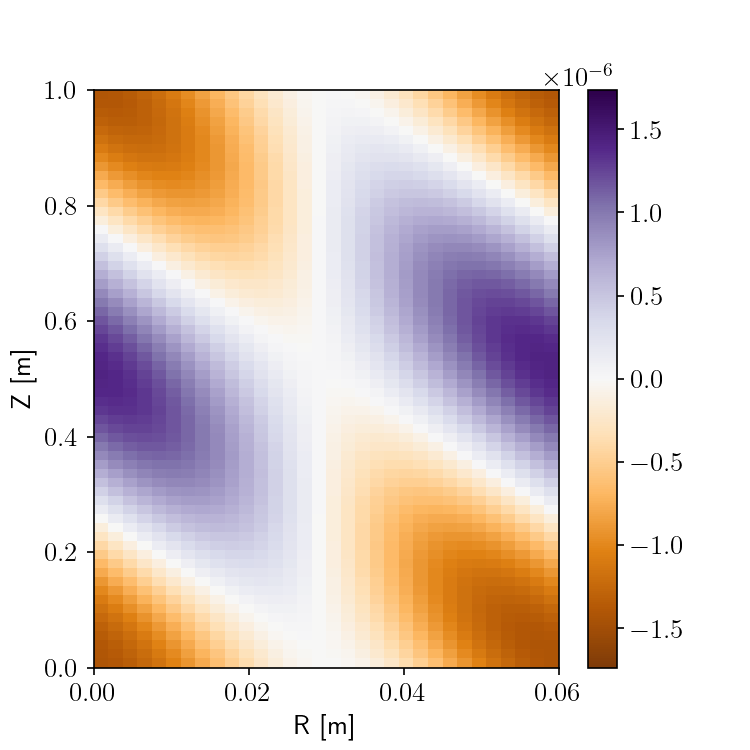
\includegraphics[width=.98\textwidth]{schemes/44_APara.png}
		\subcaption{$A_\parallel(\psi,\theta)$ at the timestep 440\\ \ }
		\label{fig:electromagneticSLAB_initialProfile_A}
	\end{subfigure}
	\begin{subfigure}[b]{0.45\textwidth}
		\centering
		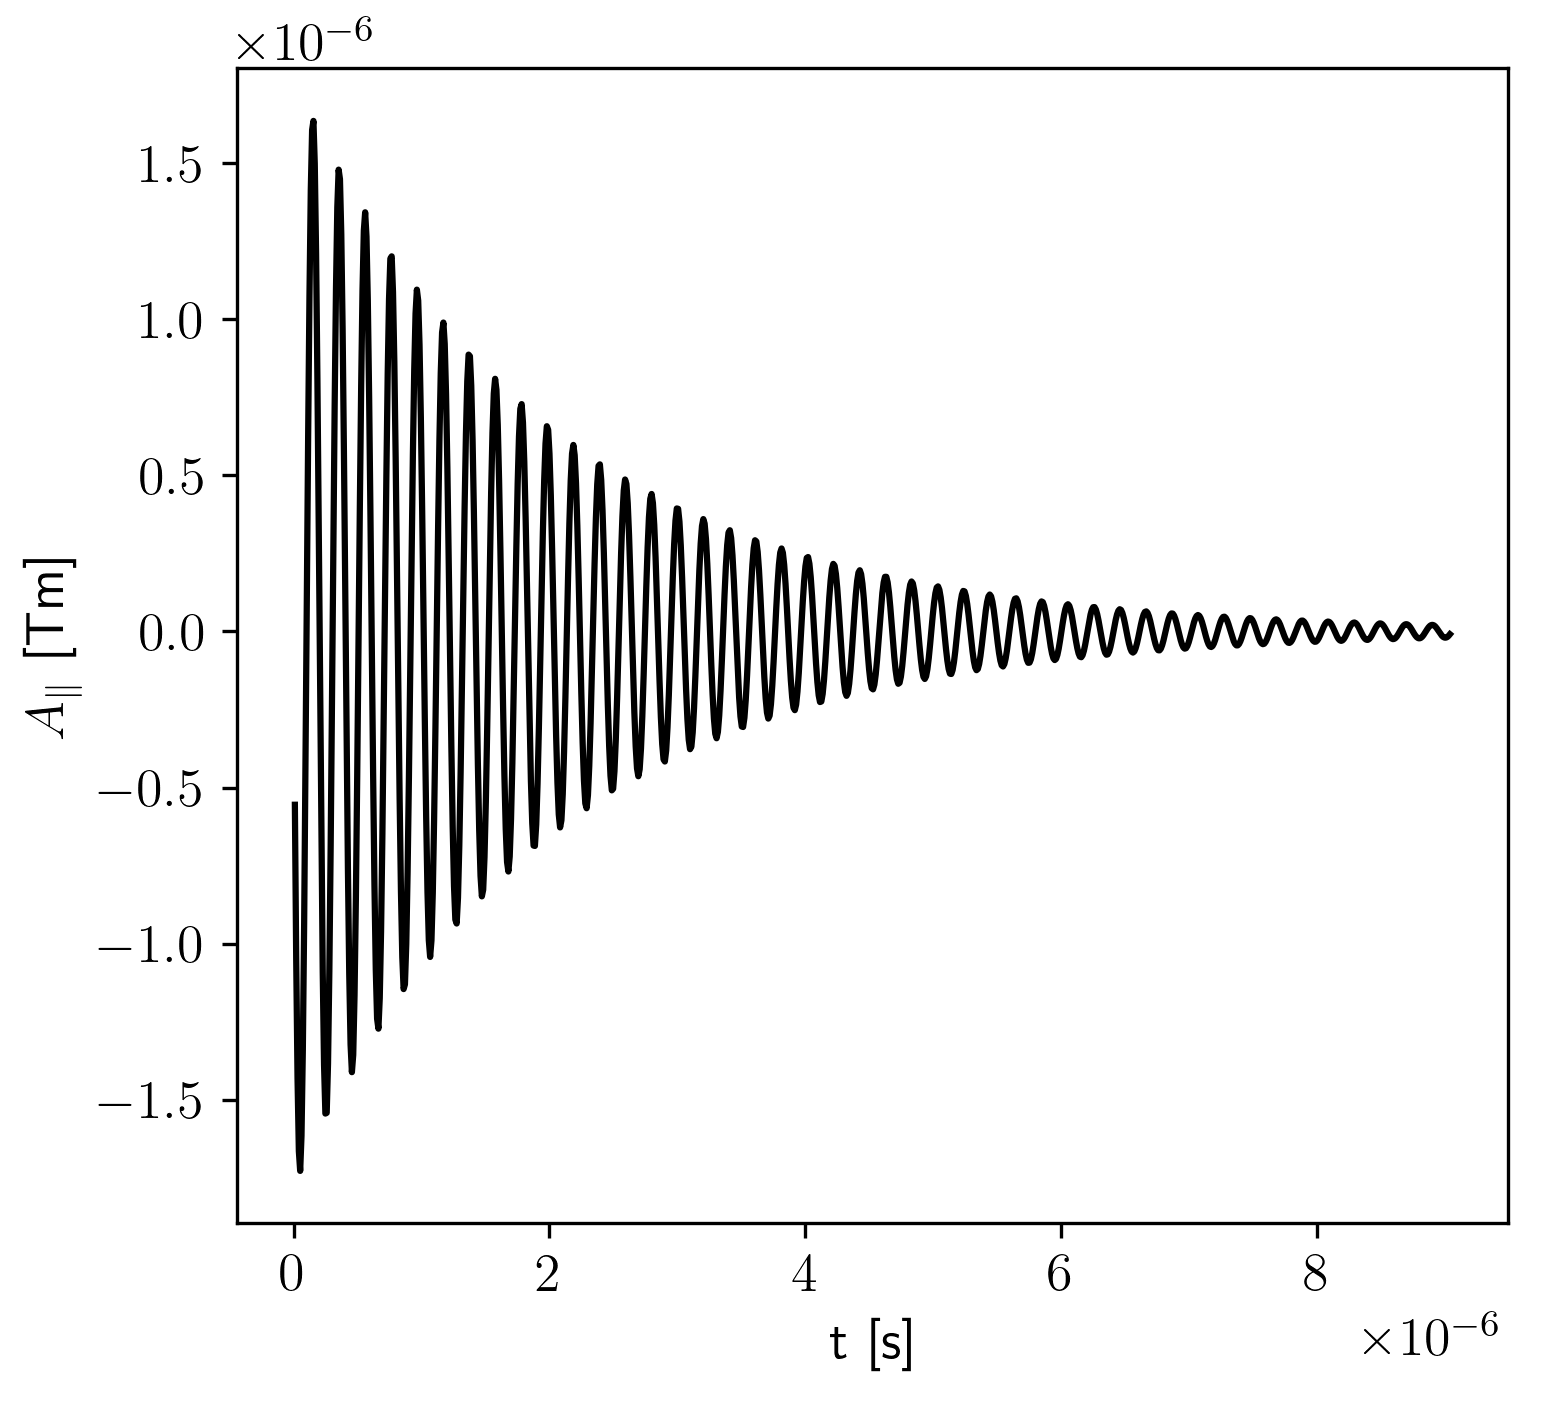
\includegraphics[width=1\textwidth]{schemes/excitedSLAB_2D_timeplot_A.png}
		\subcaption{Time evolution of $A_\parallel(t)$ in the lower left corner of the domain}
		\label{fig:electromagneticSLAB_evolution_A}
	\end{subfigure}
	\caption{Snapshot of an electromagnetic SLAB simulation on a domain with $N_\psi=32$ and $N_\theta=64$ grid points. All point at the radial center with $i_\psi^G$ are grounded.}
	\label{fig:electromagneticGroundedSLAB_system}
\end{figure}

In the simulations with a grounded line, the initial wave solution has been applied to the vorticity field $\Omega$ to prevent steep gradients and instabilities if it was done on $\Phi$ directly. Very soon, the two potentials $\Phi$ and $A_\parallel$ respond to this initial excitation and a wave profile appears as depicted in \autoref{fig:electromagneticSLAB_initialProfile_A}. The line of grounded points in the middle of the domain however breaks the wave which then smoothly lines up with the equilibrium point $\Phi_0 = 0V$ and $A_{\parallel,0} = 0Tm$ around the grounded line. At this point it may be emphasized that only the electric potential $\Phi$ is grounded, but as both potential fields are strongly coupled the grounded line affects $A_\parallel$ equally. We thus have a wave that is guided between two poloidal grounded lines (remember that the domain is periodic in radial direction) so by construction the system cannot account for radial dynamics. If we consider a point that is furthest away from the grounded line (e.g. any point on the domain boundary in the example above) we might still be able to observe some expected physical behaviour. At first glance, if we track $A_\parallel$ in one point over time as in \autoref{fig:electromagneticSLAB_evolution_A}, a decaying oscillation appears which is in line with the here dominant underdamped regime. 	

First we investigate the underdamped scenario by opposing simulation results to the expected damping rates $\lambda$ and frequencies $\omega_0$. As for the previous electromagnetic we fit the four free parameters in \autoref{eq:electromagneticSLAB_underdampedSolution} to simulation data with a nonlinear least squares method. With 1000 sample points we get a high fitting fidelity with a relative standard deviation of the order of $10^{-9}$ and the difference if the fit is performed on $\Phi$ or $A_\parallel$ has about the same magnitude. 

\begin{figure}[H]
	\centering
	\begin{subfigure}[b]{0.45\textwidth}
		\centering
		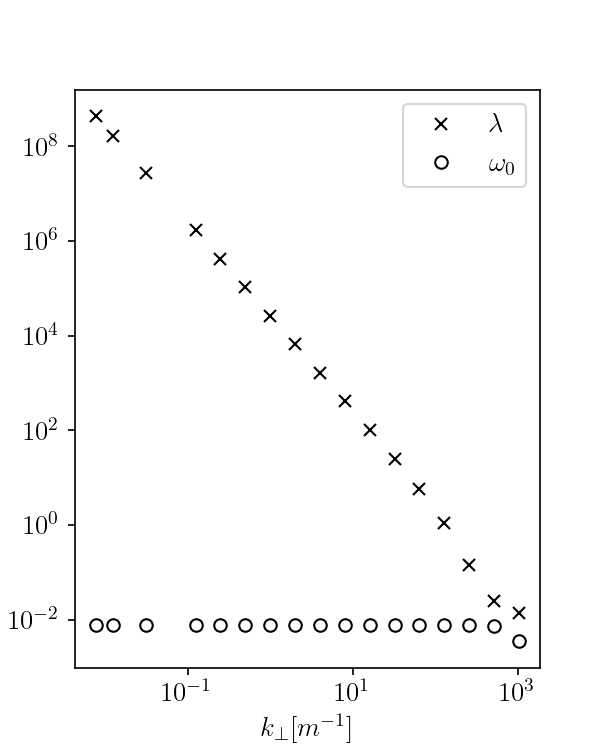
\includegraphics[width=.98\textwidth]{schemes/groundedSLABunderdampedFiterrors_k_para_fixed.png}
		\subcaption{Poloidal mode fixed to $k_\parallel = $}
		\label{fig:electromagneticSLAB_errorGrounded_kPara_fixed}
	\end{subfigure}
	\begin{subfigure}[b]{0.45\textwidth}
		\centering
		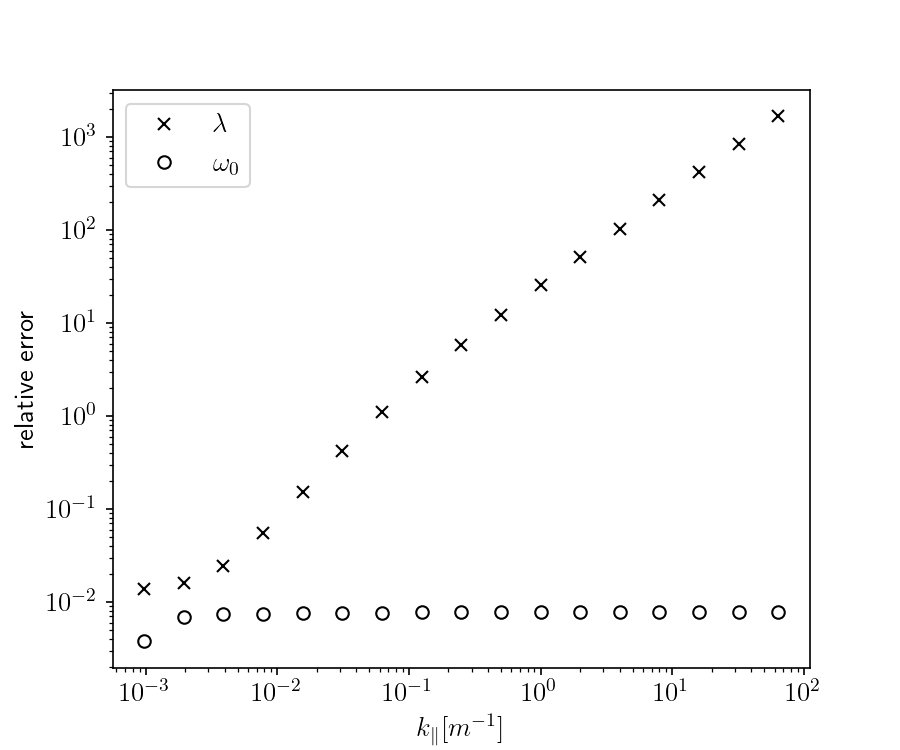
\includegraphics[width=1\textwidth]{schemes/groundedSLABunderdampedFiterrors_k_perp_fixed.png}
		\subcaption{Radial mode fixed to $k_\perp = 100m^{-1}$}
		\label{fig:electromagneticSLAB_errorGrounded_kPerp_fixed}
	\end{subfigure}
	\caption{Relative error for the fits of the frequency $\omega_0$ and the decay rate $\lambda$ on the evolution of $A_\parallel$ with respect to the expected values in a grounded electromagnetic SLAB simulation on a domain with $N_\psi=32$ and $N_\theta=64$ grid points.}
	\label{fig:electromagneticSLAB_errorGrounded}
\end{figure}






%\subsubsection{Diagonal perturbation}
%Another approach that
% 
%\autoref{eq:electromagneticSLAB_PHI} on the potential is then replaced by:
%\begin{equation*}
%	\partial_t\grad\cdot\left[\frac{m_in_i}{B^2}\grad_\perp\Phi\right] + \varepsilon \Phi= \grad\cdot\sigma_\parallel\left(-\grad_\parallel\Phi-\partial_tA\right) + \varepsilon \Phi_e
%\end{equation*}
%
%This addition naturally affects the dispersion relation and we end up with:
%\begin{equation*}
%	\omega^2+\left(i\gamma k_\perp^2 - \frac{B^2\epsilon}{m_in_ik_\perp^2}\right)\omega-v_A^2k_\parallel^2+\frac{v_A^2 \epsilon}{\sigma_\parallel}=0
%\end{equation*}
%
%This eventually changes the previously calculated frequencies and damping rates. For the overdamped case, we get:
%$$ \lambda = \frac{\gamma}{2}k_\perp^2 - \frac{B^2\epsilon}{2m_in_ik_\perp^2} \pm \sqrt{\frac{\gamma^2}{4}k_\perp^4-v_A^2k_\parallel^2}$$


\subsection{Linear transition from Alfvén to thermal electron waves}

In Sec. \ref{sec:edge_DAW}, we introduced drift-Alfvén waves. With the electromagnetic extensions, drift-waves are coupled to higher-frequency modes that transition from the Alfvén to the thermal electron speed and travel along magnetic field lines. These modes are associated with negative growth rate and usually dampen out quite fast. They can however be used to validate the electromagnetic implementation. The thought behind it is that if we reduce the system to suppress drift-waves, and run simulations with a sufficiently temporal resolution, the transition should appear in the SOLEDGE3X simulations. \\

The following simplified model (Eq. \ref{eq:VV_fourFieldModel}) is considered on the electron density $n_e$, parallel current $j_\parallel$, and the potentials $\Phi$ and $A_\parallel$: \newline

\begin{equation}
	\left\{
	\begin{aligned}
		\partial_t n_e &= \frac{1}{e}\nabla \cdot (j_\parallel \mathbf{b}) \\
		j_\parallel + \frac{\sigma_\parallel m_e}{n_e e^2} \partial_t j_\parallel  &= \sigma_\parallel \left( -\nabla_\parallel \Phi - \partial_t A_\parallel + \frac{T_e}{e} \nabla_\parallel \log(n_e) \right) \\
		\nabla \cdot \left[ \frac{m_i n_i}{B^2} \partial_t \nabla_\perp \Phi \right] &= \nabla \cdot (j_\parallel \mathbf{b}) \\
		\Delta_\perp A_\parallel &= -\mu_0 j_\parallel 
	\end{aligned}
	\right.
	\label{eq:VV_fourFieldModel}
\end{equation}

The computational domain is a 3D slab domain with periodic boundary conditions in all directions. The magnetic field is assumed to be constant in the $\theta-\varphi$ plane. The wavenumbers $k_\psi$, $k_\theta$, and $k_\varphi$ are defined by the respective dimensions of the slab. Parallel and perpendicular wavenumbers express as: \newline

\begin{align}
	k_\parallel = b_\theta k_\theta + b_\varphi k_\varphi &&& k_\perp = \sqrt{k_\psi^2 + k_\theta^2 + k_\varphi^2 - k_\parallel^2}
\end{align}

The Alfvén wave speed is given by $v_A = \frac{B_0}{\sqrt{m_u n_e \mu_0}}$ and the electron thermal speed by $v_{th,e} = \sqrt{\frac{e T_e}{m_e}}$. In the zero-resistivity limit, the dispersion relation states that we deal with a complex wave frequency, whose real component is: \newline

\begin{align}
	\label{eq:VV_dispersionRelation}
	\omega_0^2 = \frac{v_A^2}{1 + \frac{m_e}{e^2 \mu_0 n_e} k_\perp^2} k_\parallel^2 + \frac{1}{\frac{n_e \mu_0}{T_0 k_\perp^2} + \frac{1}{v_{th,e}^2}} k_\parallel^2  
\end{align}

From Eq. \ref{eq:VV_dispersionRelation}, we expect a wave in the parallel direction traveling at the Alfvén velocity for small $k_\perp$ and at the thermal electron velocity at high $k_\perp$. In the slab domain, $k_\perp$ is changed by changing the radial dimension of the domain. The results of our numerical simulations perfectly match the predictions by Dudson \cite{Dudson2021} and the numerical results obtained by Stegmeir \emph{et al.} \cite{stegmeir2019} and show the expected transition when $k_\perp$ is varied, Fig. \ref{fig:transitionSLAB}. \newline

\begin{figure}[h]\centering
	\centering
	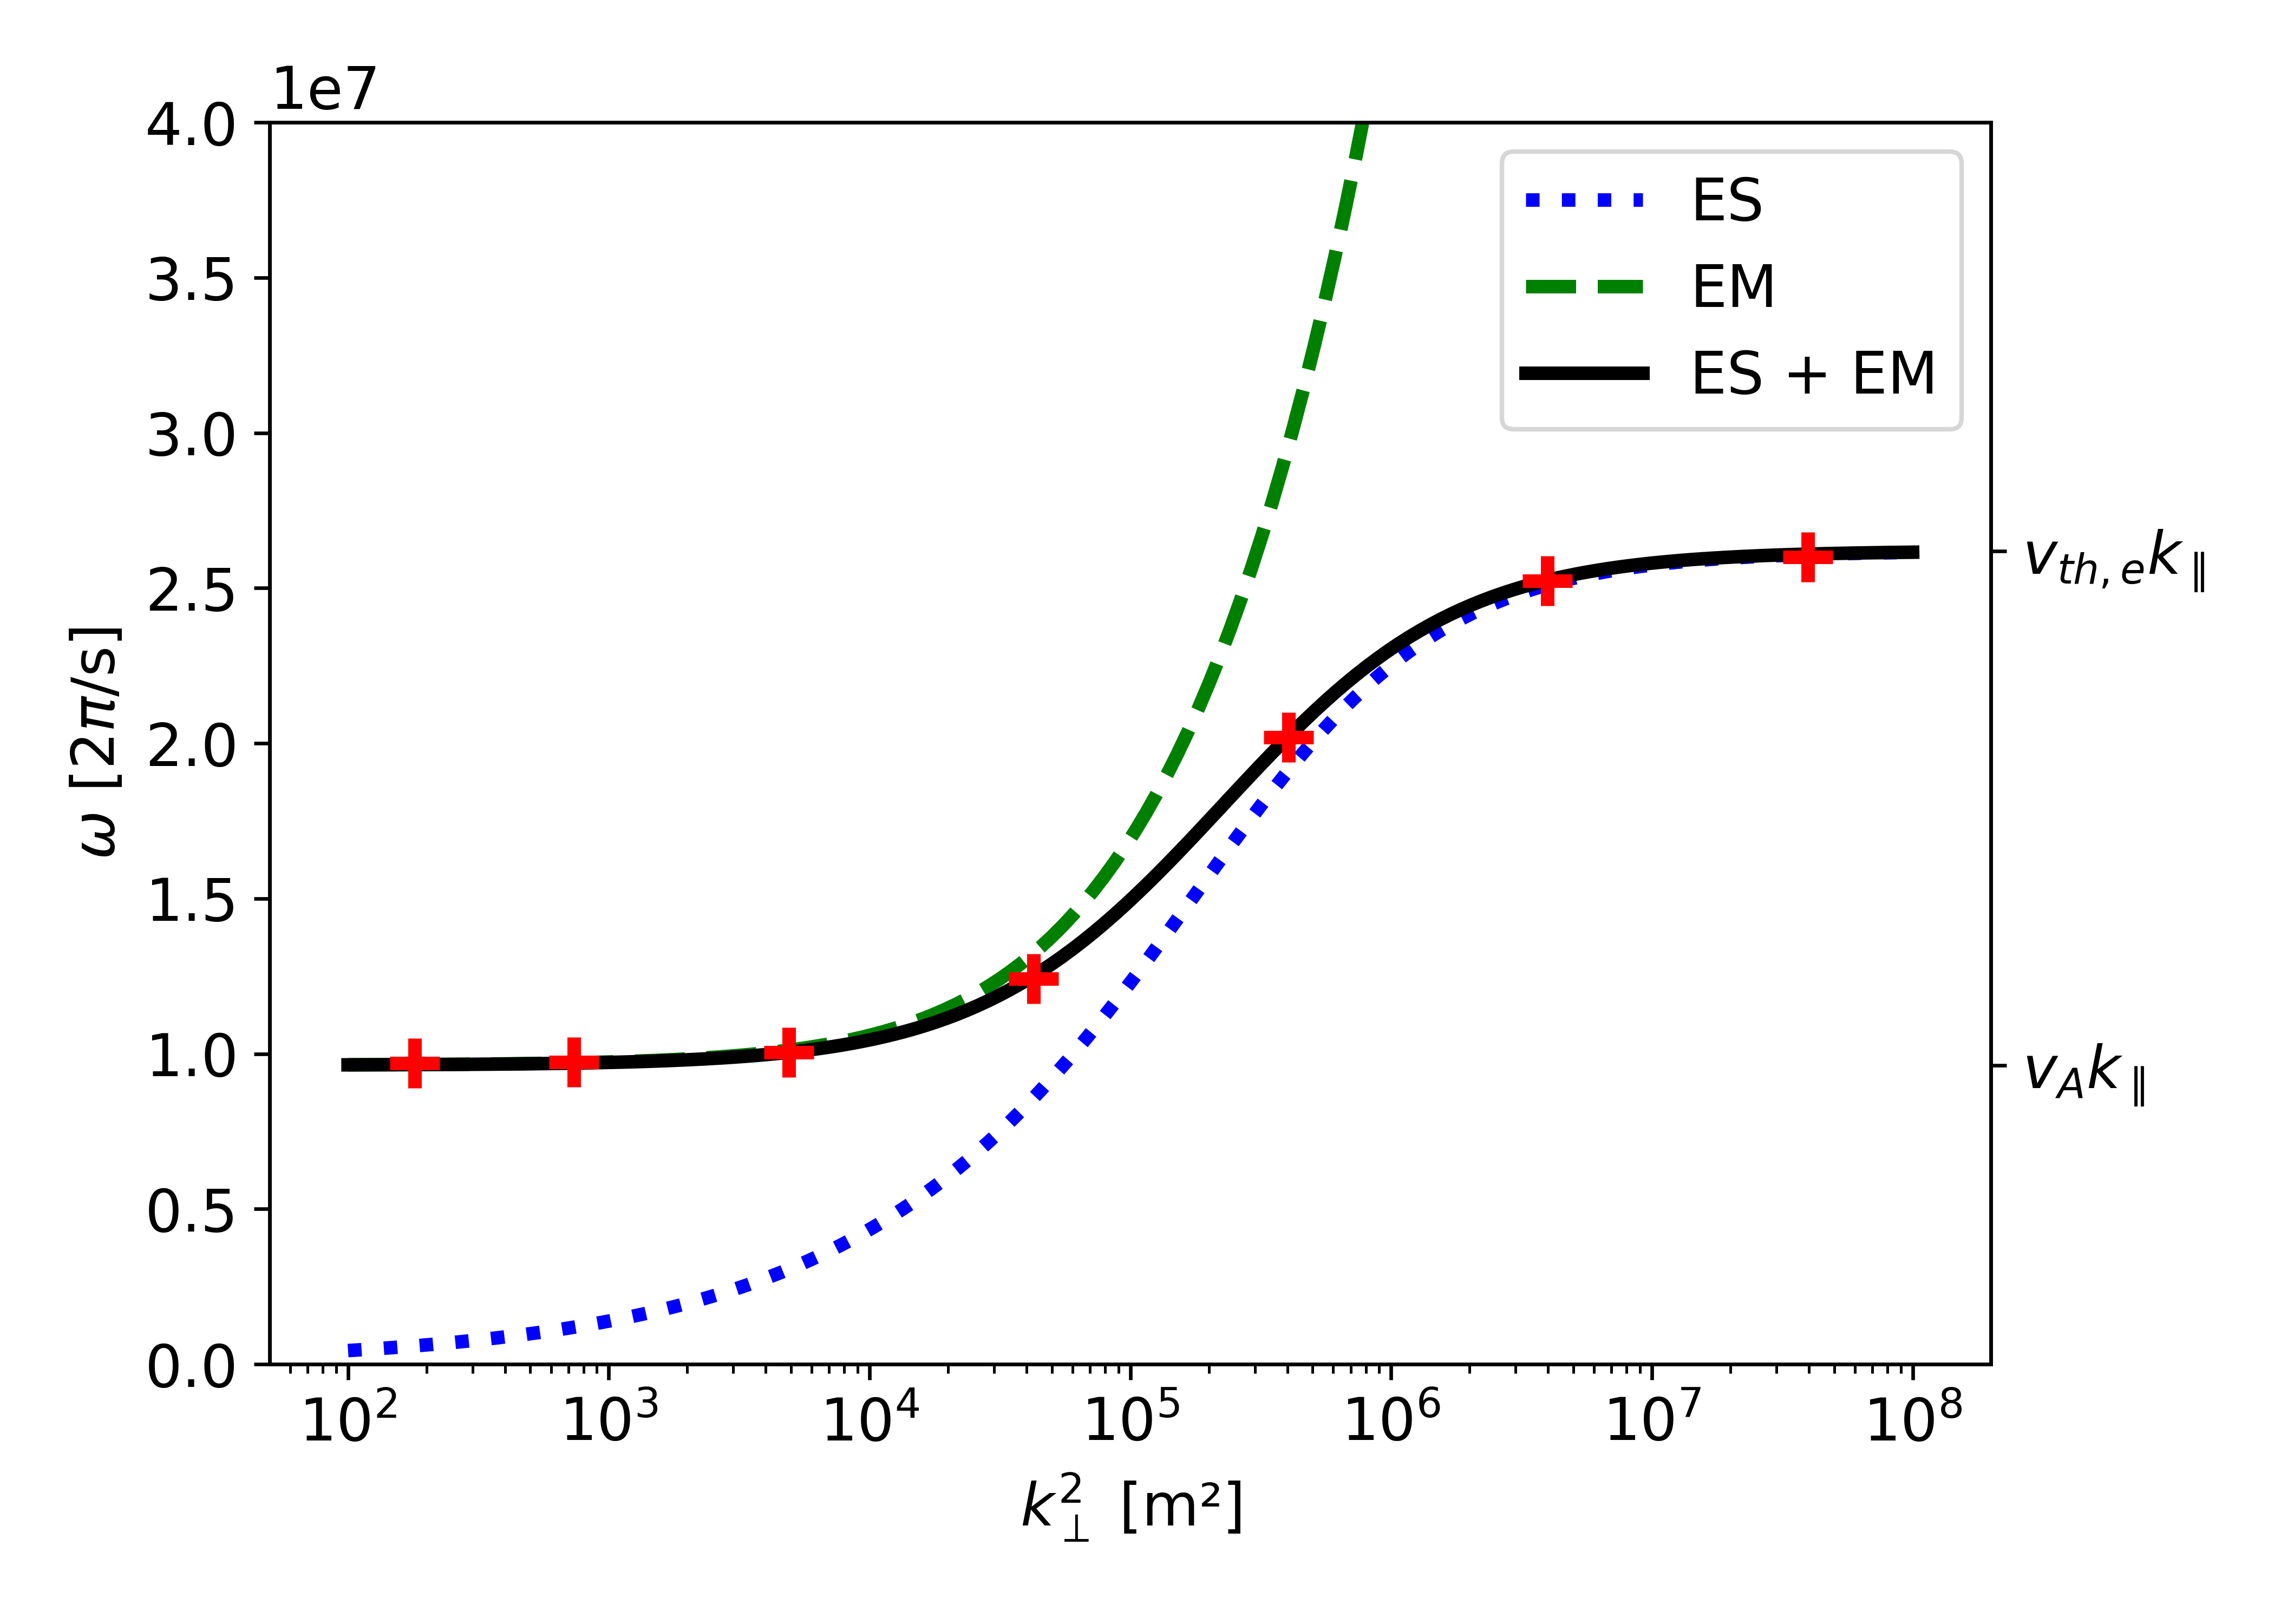
\includegraphics[width=0.7\textwidth]{schemes/transitionAlfvenThermal.png}
	\caption{Fitted wave frequencies as a function of the perpendicular wave numbers. The lines indicate the theoretical wave frequencies in the electrostatic case with finite electron mass (ES), the electromagnetic case with $m_e = 0$ (EM), and the complete electromagnetic case with electron inertia (ES + EM).}
	\label{fig:transitionSLAB}
\end{figure}




!!!! ALERNATIVE TEXT !!!!!!!
Density perturbations provoke an electromagnetic response. To this effect, we consider a standard four-field model that couples the electron density $n_e$ with the parallel current density $j_\parallel$ and both potentials $\Phi$ and $A_\parallel$. The governing equations now are: 

\begin{align}
	\grad\cdot\left[\frac{m_i n_i}{ B^2}\partial_t\grad^2_\perp\Phi\right] &= \grad\cdot(j_\parallel\mathbf{b}) \\
	\grad^2_\perp A_\parallel &= -\mu_0j_\parallel \\
	\eta_\parallel j_\parallel + \frac{ m_e}{n_ee^2} \partial_t j_\parallel  &= \left(-\grad_\parallel\Phi - \partial_t A_\parallel + T_e\grad_\parallel\log(n_e)\right) \\
	\partial_t n_e &= \frac{1}{e}\grad\cdot (j_\parallel\mathbf{b}) 
	\label{eq:fourFieldModel}
\end{align}

Its complex dispersion relation has a real and an imaginary part indicating the appearance of a decaying wave. 

\begin{equation}
	\label{eq:dispersionRelation}
	\omega_A^2 = \left(\frac{v_A^2}{1 + \frac{m_e}{e^2 \mu_0 n_e} k_\perp^2} + \frac{1}{\frac{n_e \mu_0}{T_0 k_\perp^2} + \frac{1}{v_{th,e}^2}}\right) k_\parallel^2 - \frac{\eta_\parallel^2k_\perp^4}{4\left(\mu_0+\frac{m_e}{e^2n_i}k_\perp^2\right)^2}
\end{equation}

The dispersion relation describes "shear Alfvén waves", according to which perturbations travel along magnetic field lines. In cases with high parallel conductivity, the first term dominates the dispersion relation. We then observe that the relation describes a wave in parallel direction whose velocity is bound by the Alfvén wave speed $v_A = \frac{B}{\sqrt{m_in_i\mu_0}}$ for small $k_\perp$ and by the thermal electron wave speed $v_ {th,e} = \sqrt{\frac{T_e}{m_e}}$ for large $k_\perp$. This is in line with the findings by Dudson et al \cite{Dudson2021} and reflects the need for electron inertia to avoid unphysically large speeds in the upper $k_\perp$ limit.


